\documentclass[12pt]{extarticle}

\usepackage[utf8]{inputenc}
\usepackage[T1]{fontenc}
\usepackage{lmodern}
\usepackage{graphicx}
\usepackage{color}
\usepackage{hyperref}
\usepackage{amsmath}
\usepackage{amsfonts}
\usepackage{epstopdf}
\usepackage[table]{xcolor}
\usepackage[a4paper, total={6in, 10in}]{geometry}
\usepackage{enumitem}
\usepackage[export]{adjustbox}
\usepackage{algorithm2e}

\graphicspath{ {./Figures/} }

\begin{document}

{\Large Andrew Sivaprakasam | Warm-Up 2 Write-up}

GitHub Repo: \url{https://github.com/sivaprakasaman/Numerical_Methods_BME/} 

\section{Solving a Nonlinear Single Equation}
\stepcounter{subsection}


\subsection{Bisection Method Thought Exercise}

\begin{enumerate}
\item A, B, and C demonstrate cases where there may or may not be a root between $f(x_1)$ and $f(x_m)$ when their product is greater than zero. 
**\textbf{Note:} when I drew these, I accidentally put $x_u$ instead of $x_m$
\item A and B also demonstrate that there may be multiple roots between $x_1$ and $x_u$ when their product is greater than zero.
\\
\begin{center}
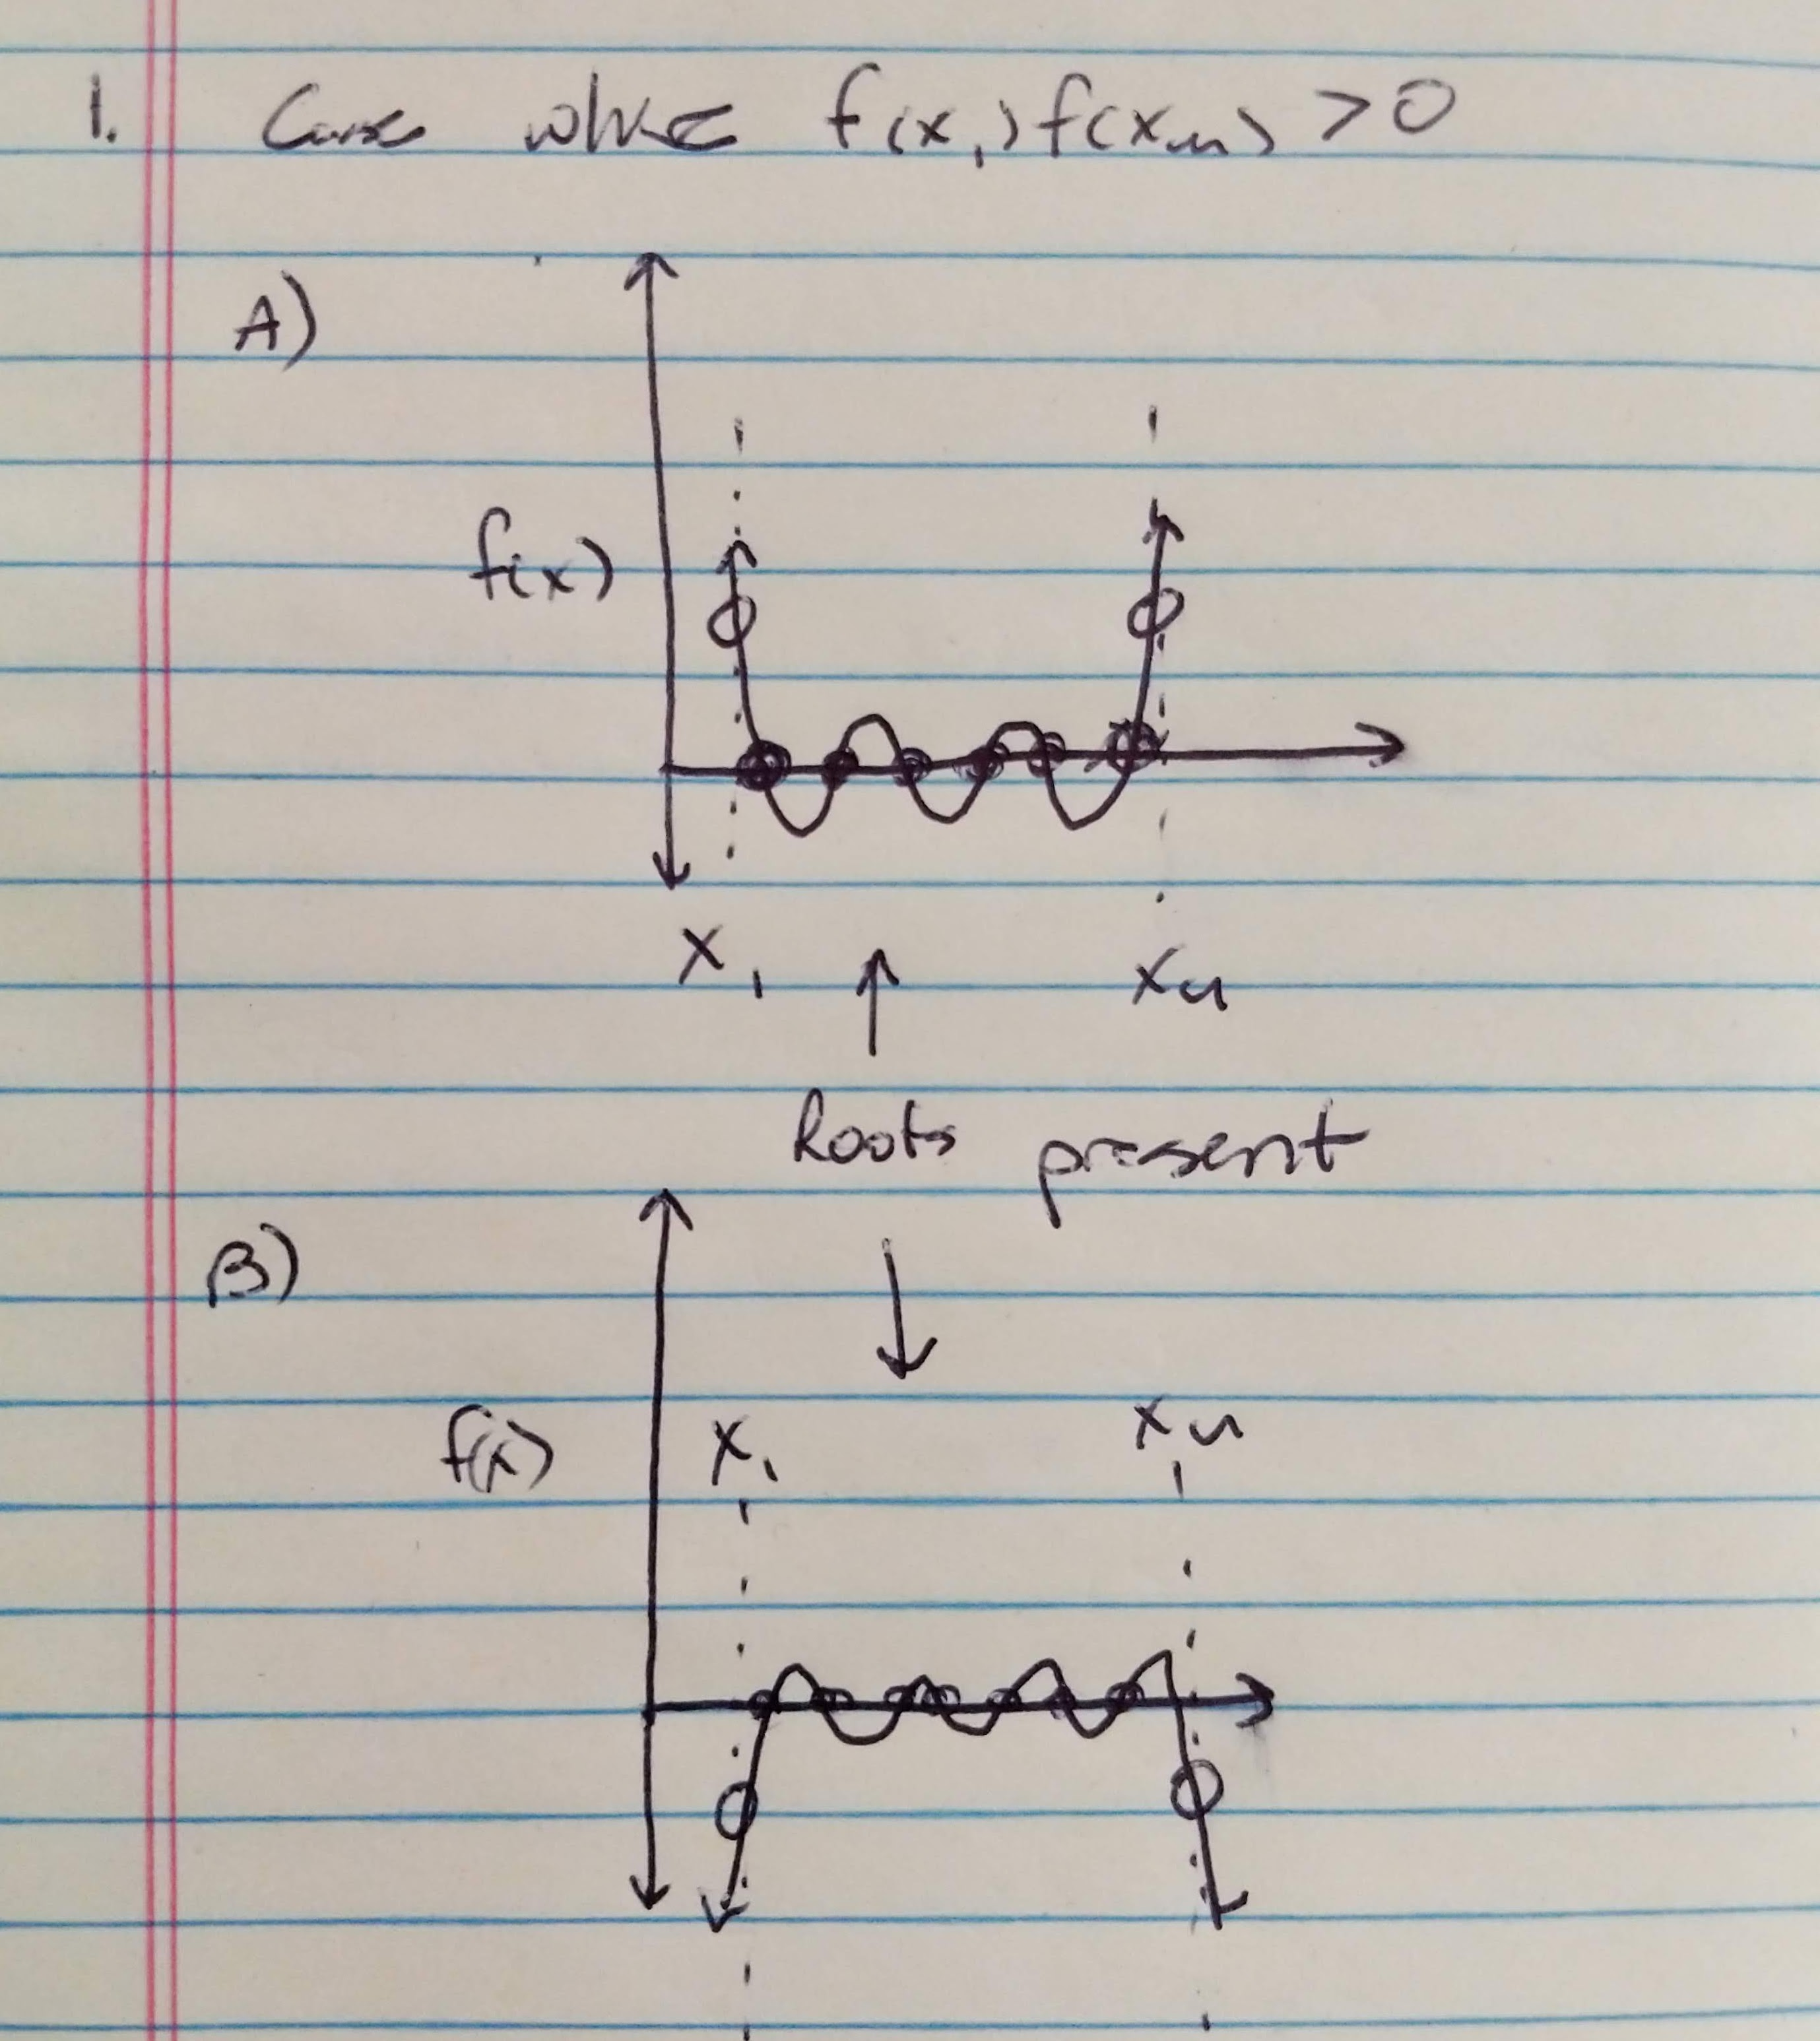
\includegraphics[width = .45\textwidth]{pic_1}
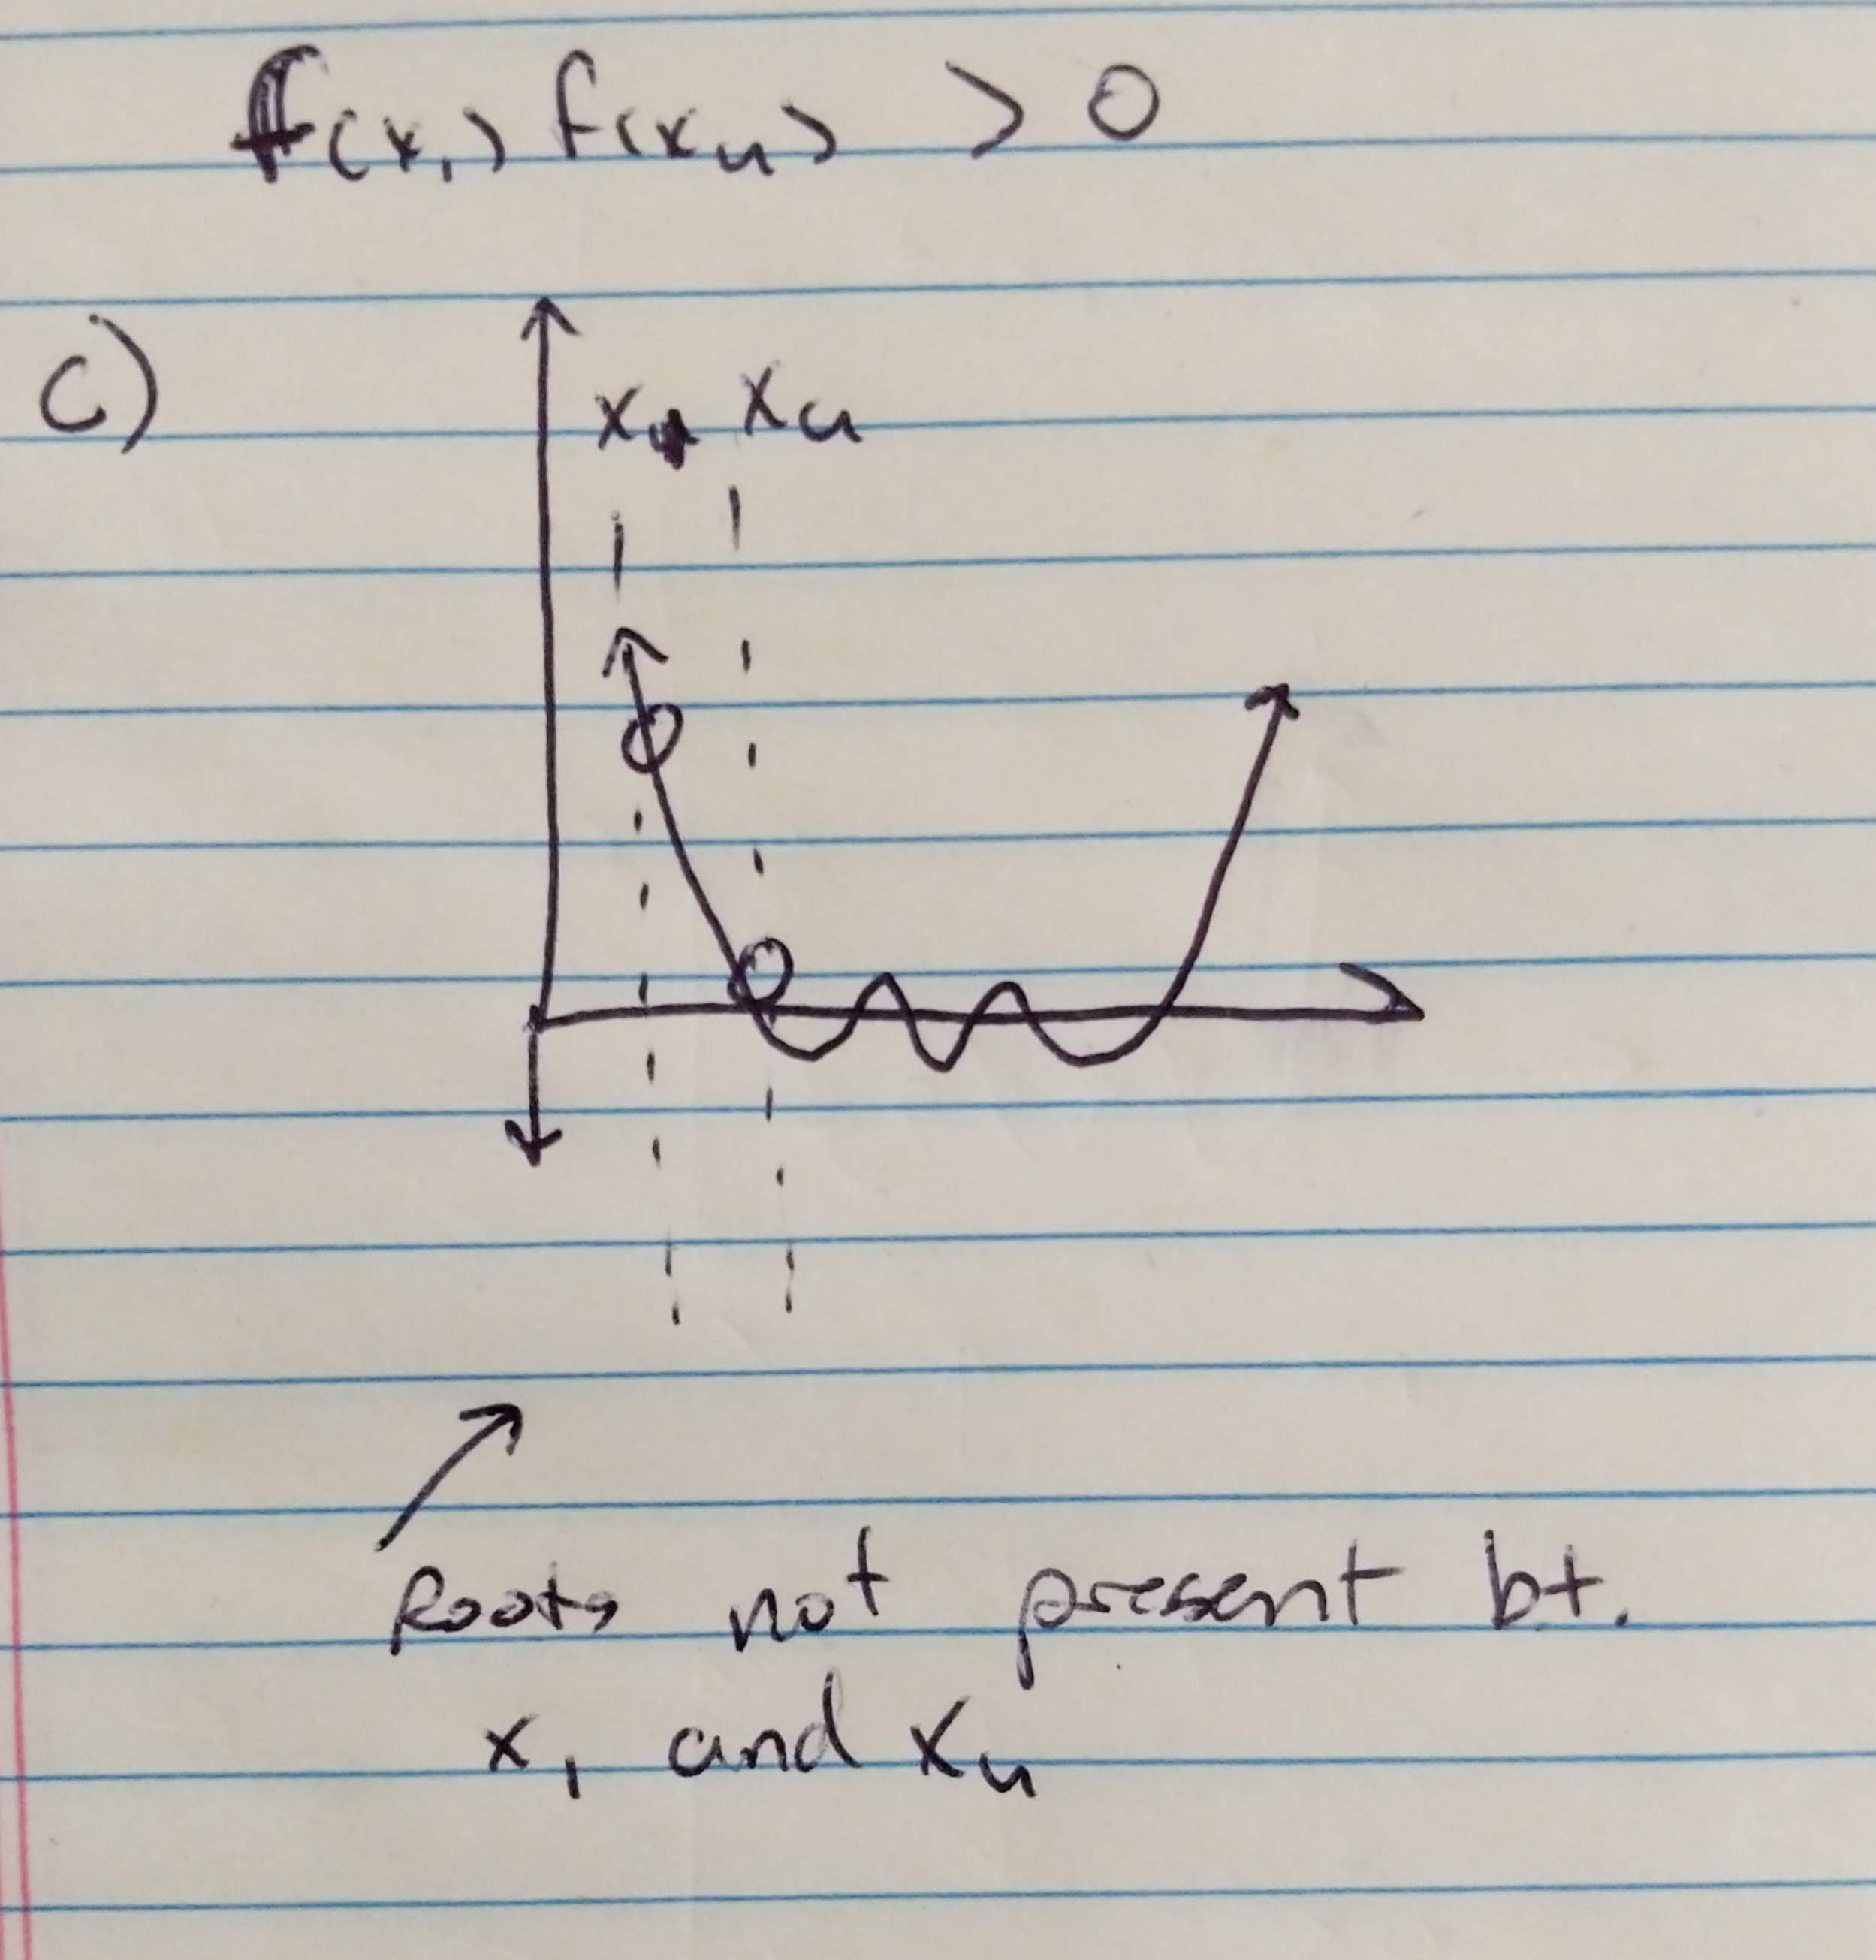
\includegraphics[width = .45\textwidth]{pic_2}
\end{center}

\item Bisection Method Flowchart:
\begin{center}
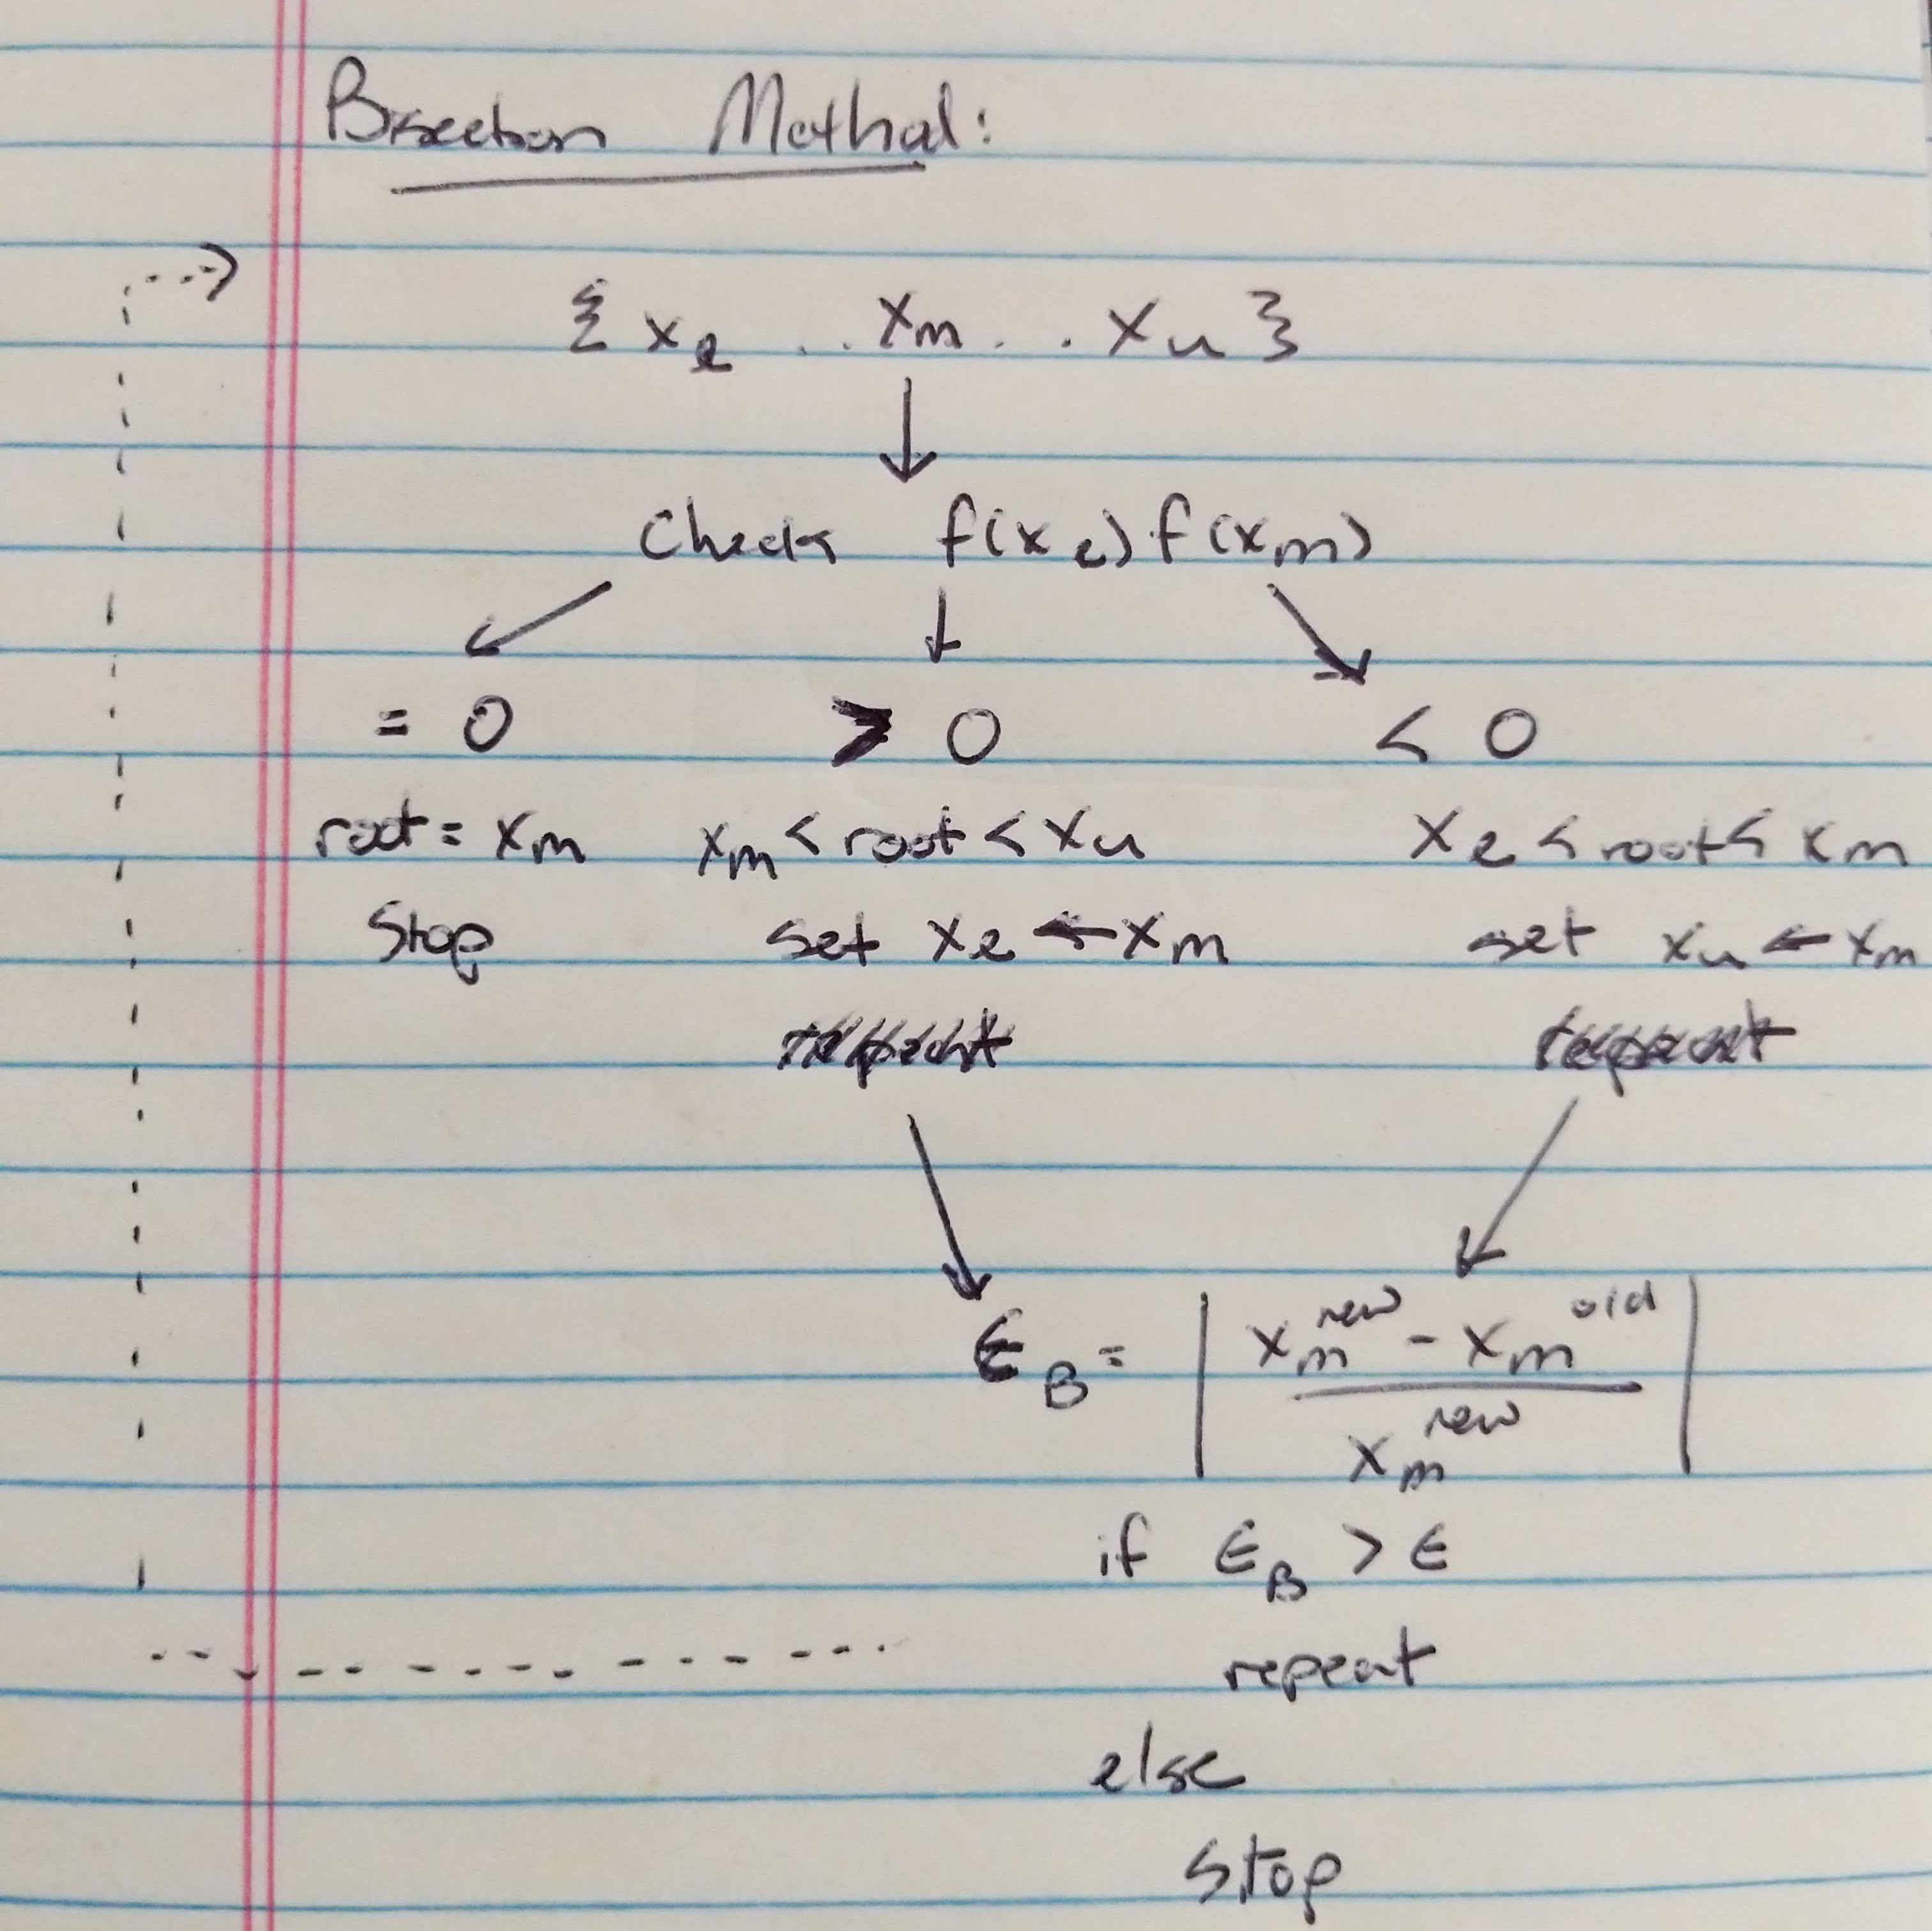
\includegraphics[width = .6\textwidth]{pic_3}
\end{center}
\end{enumerate}

\newpage




\end{document}